\documentclass{my_paper}
\usepackage{ctex}
\usepackage[textwidth=444bp,vmargin=2.5cm]{geometry}%设置页边距
\usepackage{array} %主要是增加列样式选项
\usepackage[dvipsnames]{xcolor}%颜色宏包
\usepackage{graphicx}%图片宏包
\usepackage{amsmath}%公式宏包
\usepackage[T1]{fontenc}    
\usepackage{newtxtext, newtxmath}  %两种使用Times New Roman 字体的方法
\usepackage{subfigure}
\usepackage{tabularx, booktabs} %% Load packages that you use
\usepackage{multirow} %跨行处理
\usepackage{rotating}%横向表格
\usepackage{diagbox}%斜线划分表头

\usepackage { gensymb }
% 打°符号\degree
\usepackage{framed}
\usepackage{listings}
% 代码
\usepackage{color} %red, green, blue, yellow, cyan, magenta, black, white
\usepackage[numbered,framed]{matlab-prettifier}%matlab 代码高亮
\usepackage{mdframed}%另一个边框
% matlab代码样式,使用方法为:
% \lstinputlisting[style=Matlab-editor,linewidth=\textwidth]{code.m}
% 或:
% \begin{lstlisting}[style=matlab-prettifier]
%     %code
% \end{lstlisting}
\renewenvironment{framed}[1][\hsize]
  {\MakeFramed{\hsize#1\advance\hsize-\width \FrameRestore}}%
  {\endMakeFramed}
%   修正framed环境,使之可以变长,用法:
%   \begin{framed}[1.2/textwidth]...

\usepackage{hologo}
\usepackage{gbt7714}
\bibliographystyle{gbt7714-numerical}
% 采用国标参考文献引用
\newcommand{\lunwenbiaoti}{\fontsize{15.75pt}{0}\heiti 基于滑动窗口法的云服务分析模型}
\newcommand{\zhaiyao}{\fontsize{14pt}{0}\heiti 摘要}
    
\begin{document}

\lstdefinestyle{python_style}{
 columns=fixed,
 numbers=left,                                        % 在左侧显示行号
 numberstyle=\tiny\color{gray},                       % 设定行号格式
 frame=trbl,                                        % 单线背景边框
 breaklines=true,                                     % 设定LaTeX对过长的代码行进行自动换行
 keywordstyle=\color[RGB]{40,40,255},                 % 设定关键字颜色
 numberstyle=\footnotesize\color{darkgray},
 commentstyle=\it\color[RGB]{0,96,96},                % 设置代码注释的格式
 stringstyle=\rmfamily\slshape\color[RGB]{128,0,0},   % 设置字符串格式
 showstringspaces=false,                              % 不显示字符串中的空格
 language=python,                                        % 设置语言
 basicstyle=\linespread{1.0}\fontsize{10bp}{10bp}\selectfont\ttfamily,                      % 字体字号
 %lineskip=10bp,
 %baselinestretch=1,
}
\newpage
\begin{center}
\lunwenbiaoti

\vspace{2ex}
\zhaiyao
\end{center}

云计算近些年取得了很快的发展,因此能够分析用户指标,以提供更好的服务时厂商们需要解决的问题。本文利用已知数据,首先使用滑动窗口法捕获数据趋势,利用分布的假设检验判断指标的重要程度,此外使用相关系数法排除冗余指标。为了确定预警评分的参数,使用k-means聚类的方法对用户进行划分,并使用熵权法确定各个指标的权重。

针对第一问,我们使用双滑动窗口法获得预警时间的指标变化趋势,使用基于分布的假设检验观察不同用户之间的同一参数分布是否均匀,以此判断是否为重要指标,随后使用相关系数筛选出冗余的指标。最终选出28个重要指标。

针对第二问,我们利用k-means法对于用户进行划分,并确定了划分为两类是最优的划分数量。随后使用熵权法,得出了用户画像与预警风险的数学表达。

针对第三问,利用已知数据,我们检验了模型的效果,并对附件四中的用户数据做出了预测。

针对第四问,我们使用线性拟合的方式,利用前几问中提出的判别模型,对于用户最终的流失时间做出预测。

\begin{guanjianci}
 滑动窗口法 \quad 熵权法 \quad k-means
\end{guanjianci}

%----------- 正文 ----------
%----------- 一、问题重述 ----------
\newpage
\section{一、问题重述}

\subsection{问题背景}

云计算的概念自2006年提出以来,已经有了长足的发展,渐渐成为了第四次工业革命的重要角色。其中,公有云的市场规模自2017年以来不断增长,预计到2023年将提升至2300亿元。\cite{1}公有云取得高速增长,原因在于公有云具有降本增效,弹性部署等优良特性,目前已经在远程服务,人工智能,网站部署上具有较多应用。

在此背景下,企业发展也由快速扩张的阶段转变为提升用户质量的阶段,为此云服务供应商关注各个用户的运行指标,并及时判断用户的流失风险,并且做出相应的挽留措施。

\subsection{问题重述}
经过分析整理,我们需要解决以下问题:
\begin{enumerate}
    \item 基于附件1中给出的用户指标监控值,建立筛选指标模型,在附件中所给指标里筛选出用户流失相关的重要指标,并说明指标数量和选取原因。
    \item 建立风险描述的数学模型,对每个使用者建立其用户画像,评估用户流失的风险且做出分级。
    \item 在问题一的基础上,建立用户流失的预测模型,说明流失用户的具体判别标准,重点在于流失用户的监控指标和其长期的变化趋势。利用附件中用户监控指标的监控值计算其精确率等指标,评价模型的准确性,分析相关因素的依赖性。并且使用该模型,对附件四中的用户流失情况进行判断,按照指定格式进行输出。
    \item 在问题二的基础上,预测附件四中的用户最终流失时间点所在范围。并将对应字母填入附件中。
\end{enumerate}

\section{二、问题分析}
\subsection{问题一的分析}

问题一需要我们从给出的监控数据中筛选出来关键指标,用于判断用户流失的情况。因此我们在处理数据时,需要将原始数据按用户ID归类,随后按照监控指标(metrics字段)和时序进行排列。在此之外,我们还需考虑采样率的问题,对于那些采样率不足一日一次的指标,需要进行插值填充,此外,对于那些没有参照的少数指标,我们将其剔除,认为其不是关键指标。

为了提取长期的变化趋势,我们需要忽略因为用户产生的数据波动,并且提取趋势。此后可以统计监控指标在流失的用户中变化趋势的情况,使用分布的假设检验方法来判断是否相关以及相关程度的大小,作为其重要程度的评价标准。为了尽可能地减少指标数量,使用相关系数对指标进行进一步筛选。

\subsection{问题二的分析}

在前一问的基础上,我们需要构建用户画像以归类用户,分析其特点,为此我们考虑指标分布不均衡的特点,使用聚类的方法对于指标为共性的用户归为一类。随后利用熵权法求取各个监控指标的权重,以量化用户画像以及风险特征。

\subsection{问题三的分析}
基于附件一和附件三给出的数据,利用重要指标的长期变化趋势来构建用户的流失预测模型。构建模型后需要利用附件一和三中的数据检验其准确度。具体做法为打乱数据,输入模型中,判断输出结果与正常的差异,通过精确率、召回率及F1-score来评价该模型准确性。最后利用附件四中没有标签的数据进行预测。

\subsection{问题四的分析}
我们在问题三中已经建立起了判断用户是否会流失的模型,第四问的模型预测就是根据现有的指标数据对指标的变化进行预测,再对预测后的指标利用问题二、三的模型进行打分,再与用户流失的分界值作比较。由此对一个用户每隔半个月(15天)进行一次打分,知道分数低于流失边界,以此获得用户流失的大概时间段。
%----------- 三、模型假设 ----------
\section{三、模型假设}
%使用代码片段:、jiashe%
\begin{enumerate}
    \item 假设数据真实可靠,具有较高的可信度。
    \item 监控指标的分度值适合,不会忽略较小的趋势


\end{enumerate}

%----------- 四、符号说明 ----------
\section{四、符号说明}
%使用三线表格最好~

\subsection{符号说明}
以下是本文使用的符号以及含义:
\begin{table}[h]%htbp表示的意思是latex会尽量满足排在前面的浮动格式,就是h-t-b-p这个顺序,让排版的效果尽量好。
    \centering
    \begin{tabular}{p{2.0cm}<{\centering}p{9.0cm}<{\centering}p{2.0cm}<{\centering}}
 %指定单元格宽度, 并且水平居中。
    \hline
    符号 & 说明 & 单位 \\ %换行 
    \hline
    $D$ & 监控指标 & /\\
    $U$ & 用户    & / \\
    $k$ & 斜率   & /\\
    
    \hline
    \end{tabular}
\end{table}

%----------- 五、模型的建立与求解 ----------
\section{五、模型的建立与求解}

以下将对提出的四个问题进行建模求解。

\subsection{基于分布的重要指标筛选模型}

附件1中给出了250名用户的云服务监控指标,我们首先对数据进行预处理,包括读取整理,填补缺失值,可视化分析等步骤。在得到可以利用的数据后,为了提取各个监控指标的长期变化趋势,我们使用双滑动窗口法\cite{2}来捕获趋势滤除噪声,该趋势具有自然的分段特性。随后统计了在各个种类的监控指标中产生预警的情况,利用预警时刻的趋势分布,使用分布的假设检验来判断用户流失相关的重要指标。这部分的工作可以归结为图\ref{p1}。

\subsubsection{数据预处理}

我们对监控指标按用户id和类别进行整理,观察得到以下特点:
\begin{enumerate}
    \item 用户具有的数据指标分布不均,每个用户与其他用户的指标组合都较为不同。我们对以附件一为例,对用户具有的指标做了统计,展现为以下结果:
    \begin {figure}[h]
    \centering % 居中显示
    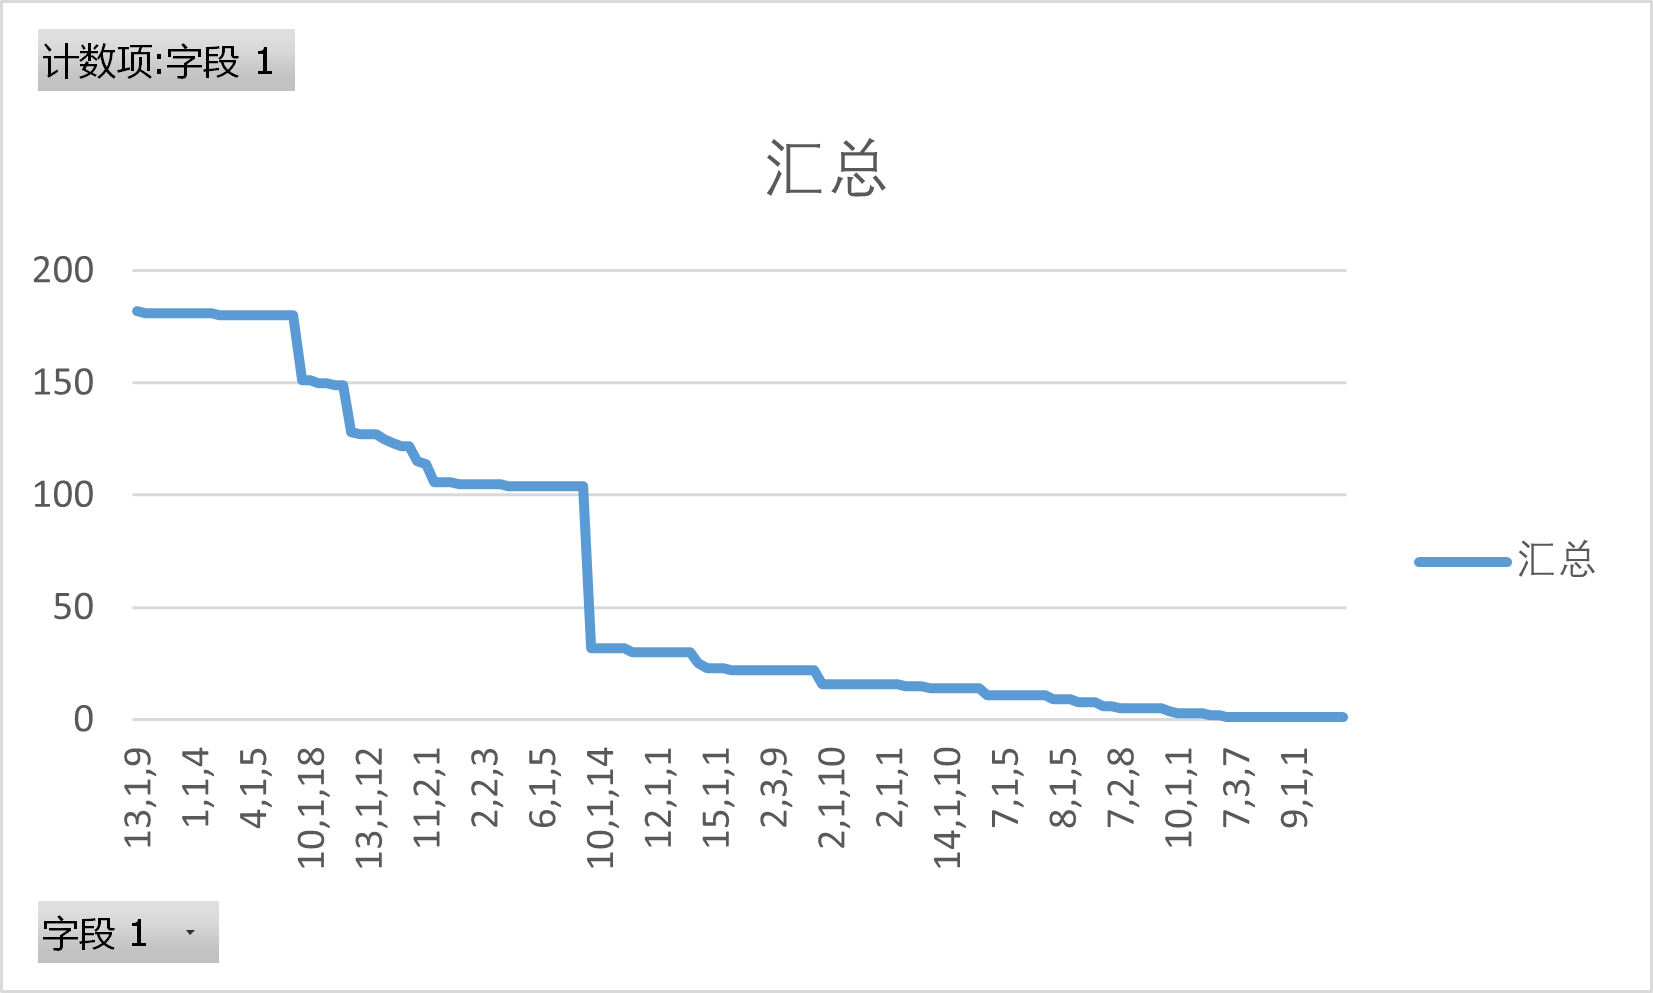
\includegraphics[width=\textwidth]{zhibiao.png}
    \caption{所有用户的指标统计(按数量排列)} % 标题
    \label{five}
    \end {figure}
    \item 统一用户的不同指标分布的时间和采样间隔均有不同,在分析数据趋势时,需要进行插值,寻找共同区间进行相关性分析等操作。
\end{enumerate}

\subsubsection{基于滑动窗口法的指标趋势识别}

根据云服务的特点,用户的监控指标发生趋势性变化时才被认为是判定为流失。而使用拟合或是差分等手段对数据进行直接处理,则会分别模糊整体趋势以及受局部噪声干扰的问题。综合这两种方法的特点,我们从常用的数据挖掘方法中使用双滑动窗口法,来判断每个用户、每一指标的变化趋势。

用户的某一监控指标$D_{ijk},(i\in \{1,2,3\})$按照一定的采样率进行记录,我们若使用$\{t_1,t_2,t_3,\cdots,t_n\}$代表数据记录的时间点,使用$\{d^1,d^2,d^3,\cdots,d^n\}$代表第$i$个时间点下的监控指标。为了判断这一序列的变化趋势,采用最小二乘法计算其斜率,计算方法由式(\ref{erc})给出:

\begin{equation}
    \left(\begin{array}{l}k \\b\end{array}\right)=\left(\boldsymbol{D}^{\mathrm{T}} \boldsymbol{D}\right)^{-1} \boldsymbol{D}^{\mathrm{T}} \cdot \boldsymbol{T}
\label{erc}
\end{equation}

所得k值由于是区间的变化趋势,较好的减弱了噪声的影响,我们根据k值来判断变化趋势。引入趋势变化基元,分为平直基元上升基元和下降基元三种,对应图(\ref{jiyuan})的三种情况。

\begin {figure}[h]
\centering % 居中显示
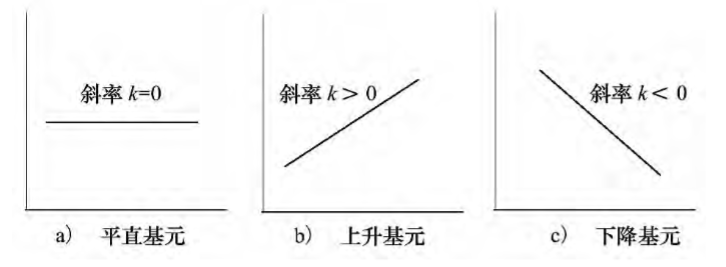
\includegraphics[width=0.8\textwidth]{jiyuan.png}
\caption{三种基元示意图} % 标题
\label{jiyuan}
\end {figure}

三种基元根据$k$ 的大小进行判断,设立$k_s$ 作为趋势阈值,当$k$ 大于$k_s$ 时识别为上升基元,小
于$k_s$ 时识别为下降基元,当$-k_s < k < k_s $时判断是否满足长时变化阈值$\Delta_s$。趋势阈值$k_s$ 和长时
变化阈值$\Delta_s$ 由我们所分析的数据的方差等统计量乘以系数得到,或是查阅相关资料得知。$k_s$ 的引
入有效减少了错误检测平稳基元的情况。$\Delta_s$ 引入是为了判断长时间的监控指标变化,式(\ref{3})满足,则
序列趋势识别为上升或者下降。

\begin{equation}
    |k\cdot m|>\Delta_s
    \label{3}
    \end{equation}

    综上所述,利用$k$值来识别基元种类的方法由图(\ref{jyz})所示。

    \begin {figure}[h]
    \centering % 居中显示
    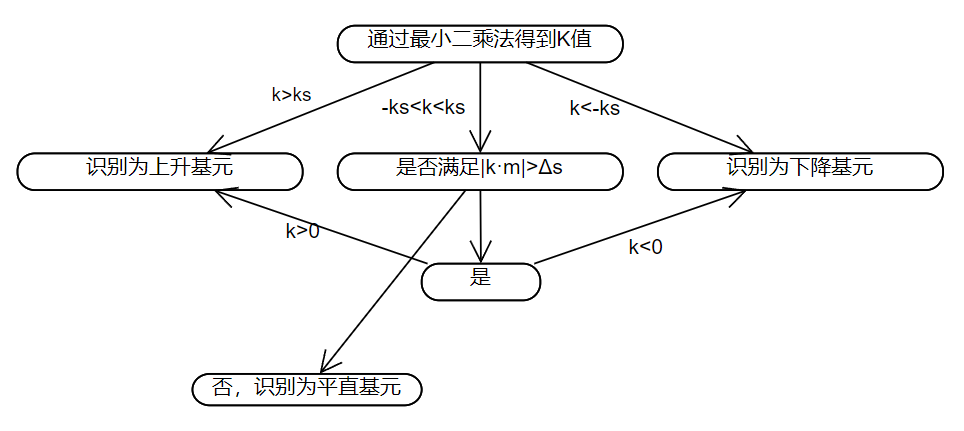
\includegraphics[width=0.8\textwidth]{jiyuanz.png}
    \caption{基元识别流程图} % 标题
    \label{jyz}
    \end {figure}

为了尽可能减少噪声影响的同时还可以检测趋势,使用双窗口滑动\cite{2}的方式来兼顾两个要求。构建一个滑动窗口和一个固定窗口,滑动窗口的大小保持不变,固定窗口的大小会发生变化。在初始状态下,滑动窗口和固定窗口的大小均为$m$,在算法执行过程中,滑动窗口向序列前方滑动来分析局部趋势$k_h$,固定窗口扩大相同长度来记录分析整体趋势$k_g$。窗口的行为由当前窗口分析出的基元结果来决定。

当窗口内的基元种类为上升或者下降时,此时滑动窗口向前移动一个单位,固定窗口相应扩大,再次考察移动后的$k_h$值,直至识别出基元的类型产生变化。当基元的类型产生变化时,根据$k_g$将固定窗口中的基元识别结果输出,作为该段的基元检测类型。同时将固定窗口的起始点位置移动置滑动窗口的起始点处,窗口大小重置为原长度$m$。

若窗口内的基元种类时平直状态时,滑动窗口向前移动一个单位,固定窗口同样扩大相同长度来记录分析整体趋势,此时需要考虑滑动窗口的$k_h$与固定窗口中的$k_g$之间的差值$\Delta k$,此时对应以下三种情况:

\begin{enumerate}
    \item $|k|>k_s$时将固定窗口中的数据识别为平直基元,并将固定窗口的数据识别为平直趋势,将固定窗口的长度重置,起点移动至滑动窗口的起点处。
    \item $|k|>k_s$且$\Delta k > \Delta s$则将固定窗口的行为识别为上升或下降,随后转至上一状态。
    \item $|k|>k_s$且$\Delta k < \Delta s$则继续向前滑动,扩大固定窗口的大小。
\end{enumerate}

综合上述过程,总结序列基元识别的状态转移图如图(\ref{slide})所示。

\begin {figure}[h]
\centering % 居中显示
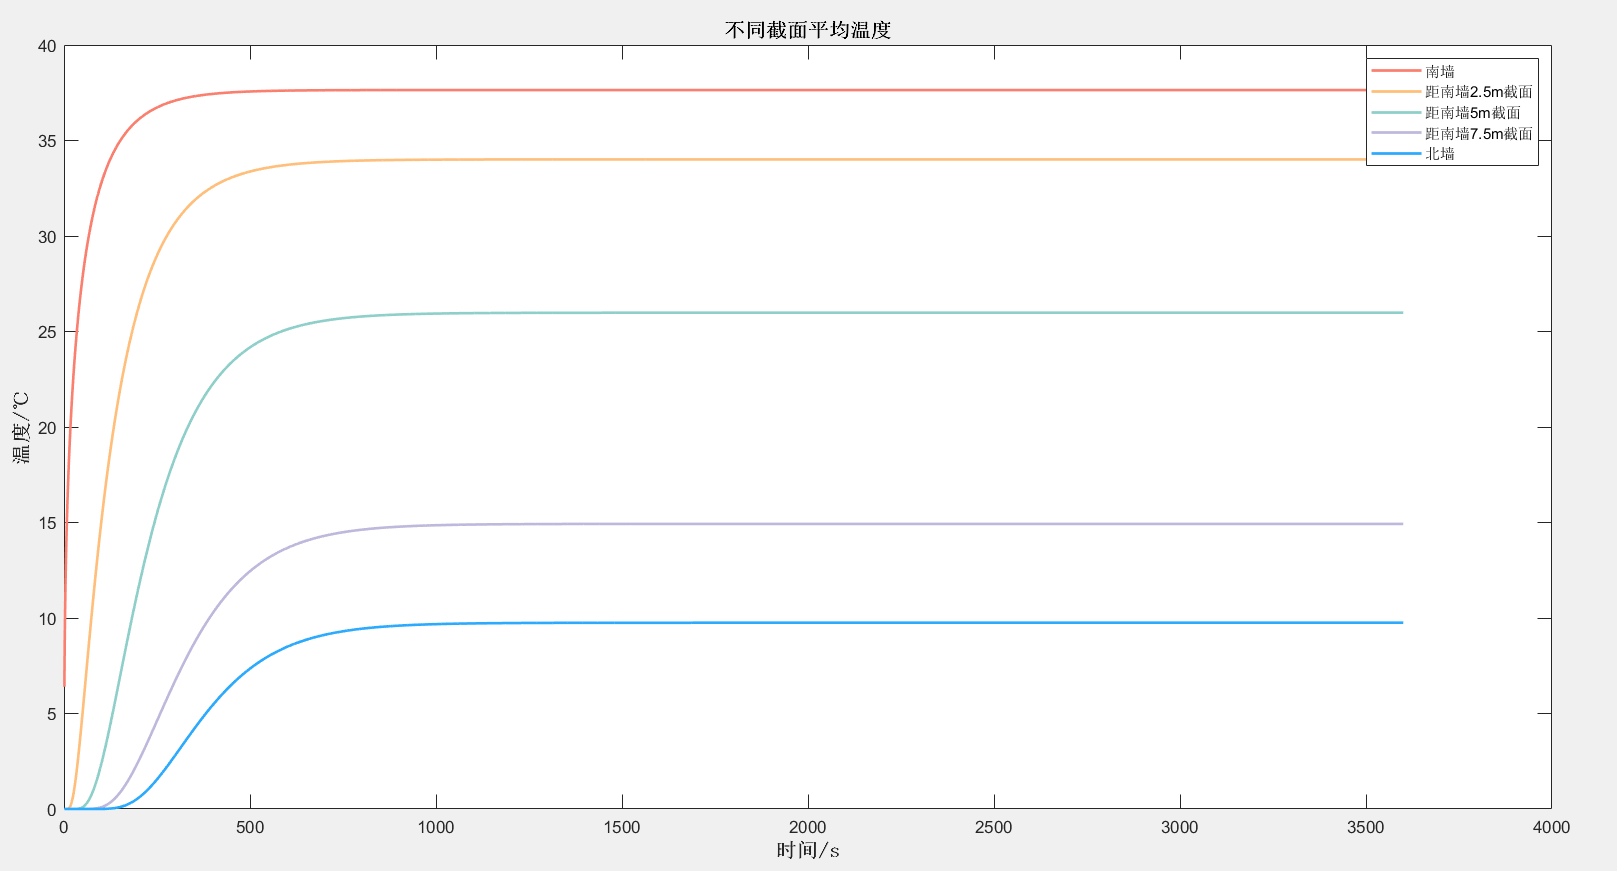
\includegraphics[width=\textwidth]{slide.png}
\caption{双滑窗移动状态转移图} % 标题
\label{slide}
\end {figure}

至此,我们对于用户$U_h,h\in\{1,2,\cdots ,250\}$存在的监控指标$D_{ijk}$都通过滑窗处理,得到按照变化趋势分段的监控指标序列。鉴于这250名用户都具有被预警的经历,因此我们统计了预警时刻所在的指标$D_{ijk}$的趋势分布情况。接下来,我们利用这一分布情况进行分布的假设检验,验证某个指标是否与用户流失相关。

\subsubsection{分布假设检验分析相关性}

在前面工作的基础上,我们得到了每个监控指标在预警时的趋势分布。对于156种监控指标$D$而言,发生预警时的趋势可以统计为一个后验概率$P_{(i,j,k)}$,利用该后验概率,可以观察到这一指标$D_{(i,j,k)}$变化趋势同发生流失风险预警与否这一时间的相关性。

我们提出如下假设:
\begin{equation}
    H_0 : P_{l} = P(Q_{(i,j,k)}=q_l) = \frac{1}{3} ,\quad \text{其中} \quad q_l \in\{\text{上升,下降,不变}\}
\end{equation}
这是由于如果某一指标的变化趋势同预警没有关系,也就是说不是重要指标的话,在预警时趋势并不会有分布不均的情况,因此各个趋势出现的概率是相同的。

我们选取统计量$\chi ^2$进行假设检验,如下所示:
\begin{equation}
    \chi ^2 = \sum_{i=1}^3\frac{(f_i-nP_i)^2}{nP_i}
    \label{chi}
\end{equation}
,其中$f_i$为发生预警时各个趋势的数量,$n$为该监控指标$D$对应的预警次数。

对于假设$H_0$的拒绝域而言,依据皮尔逊卡方检验的规则\cite{3},式(\ref{chi})的统计量服从于$K-r-1$的$\chi ^2$分布,其中$K$为类别数目,$r$为未知参数个数。因此,原假设$H_0$的拒绝域为:

\begin{equation}
   W = \{\chi^2 \geq  \chi^2_{0.05}(2) \}
\label{}
\end{equation}

对于任意观测指标而言,当其处于拒绝域内时,则认为原假设$H_0$不成立,也就是说该观测指标同预警相关,反映出该指标为用户流失的重要指标。

在筛选出一部分用户的流失指标$D'$后,为了能够减少分析指标的数目,我们对$D'$中的指标进行相关性分析,对那些相关性较大的指标进行简化。具体步骤如下:
\begin{enumerate}
    \item 依次选取附件1中的用户$U$
    \item 两两选取观测时间具有重合的观测指标$D'$,计算其协方差。假设两指标分别为$x$和$y$,则在两指标共同覆盖的区间内,其相关系数$\rho$计算方法由式(\ref{xg})给出:
    \begin{align}
    cov(x,y) &= \frac{\sum_{i=1}^N(x_i-\bar{x} )(y_i-\bar{y})}{N-1}\\
    \rho_{xy} &= \frac{cov(x,y)}{\sigma_x\cdot\sigma_y}
    \label{xg}
    \end{align}
    \item 对每一用户都计算相关系数$\rho$,并统计不同用户同一指标对之间的相关系数均值$\bar{\rho}$
    \item 对于某一指标对而言,若其$\bar{\rho} > \rho_0$时,认为两变量高度相关。为了在$x$和$y$之间选取一个,我们比较$\chi_x$和$\chi_y$,最终保留最大的那个。
    \item 记录每个最终保留的监控指标,构成最终监控指标的集合$D''$,作为与用户流失的相关指标。

\end{enumerate}


\subsubsection{模型求解与结果}
我们首先利用滑动窗口法求解得用户趋势,以用户User9的$(1,1,1)$和$(1,1,3)$指标进行展示。
\begin{figure}[htbp]
    \centering  %居中
    \subfigure[指标$ (1,1,1) $]{   %第一张子图
    \begin{minipage}{0.4\textwidth}%大小总和超过textwidth则自动换行
    \centering    %子图居中
    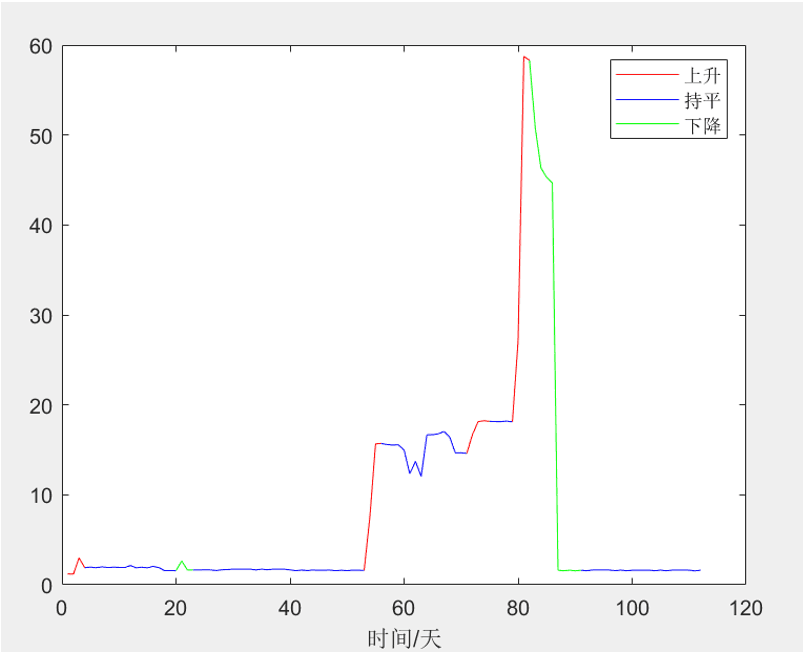
\includegraphics[width=\textwidth]{111.png}  %设置图片的输出大小倍数,这里是0.5倍大小输出
    \end{minipage}
    }
    \subfigure[指标$(1,1,3)$]{ %第二张子图
    \begin{minipage}{0.4\textwidth}
    \centering    %子图居中
    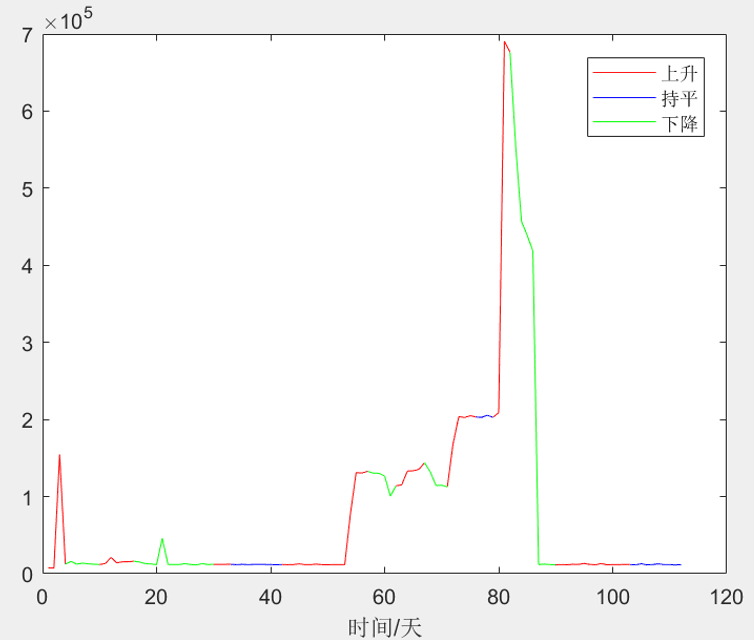
\includegraphics[width=\textwidth]{113.png}%以pic.jpg的0.5倍大小输出
    \end{minipage}
    }
    

    \caption{用户User9的部分指标趋势图}    %大图名称
    \label{fig:1}    %图片引用标记
\end{figure}
可见采用双滑动窗口法较好的捕获了长期趋势。

由于选取的指标较多,无法一一展示求解结果,因此选取在图一中统计最多的指标$(13,1,9)$进行分析,我们利用下表展示求解过程。
\begin{table}[htb]
\centering
\caption{指标$(13,1,9)$的假设检验求解}
\begin{tabular}{cccccc}
\toprule
变化趋势&$f_i$&$ p_i $&$ np_i $&$ f_i-np_i $&$ \chi^2 $ \\ \midrule
上升& 118 &  $\frac{1}{3}$&166&-48&13.88 \\
持平& 6 &  $\frac{1}{3}$&166&-160&154.22 \\
下降& 373 &  $\frac{1}{3}$&166&207&258.13 \\
$\sum$ & 497 &&&&$426.23>11.071$ \\
\bottomrule
  \end{tabular}
\label{label}
\end{table}

由上表的结果分析可知$\chi ^2 > \chi^2_{0.05}(2)$因此我们认为该$(13,1,9)$为重要指标。

利用相同的方法,我们确定了重要监控指标共有28项:
\begin{itemize}
    \item "1,1,1"	"1,1,2"	"1,1,3"	"1,1,4"	
    \item "2,2,2"	"2,2,3"	"2,2,5"	"2,2,6"	"2,2,8"	"2,2,9" "2,2,11" "2,2,12"	
    \item "4,1,1"	"4,1,2"	"4,1,3"	"4,1,4"	"4,1,5"	"4,2,1"	"4,2,2"	"4,2,3"	"4,2,4"	"4,2,5"
    \item "13,1,11"	"13,1,4"	"13,1,6"	"13,1,7"	"13,1,8"	"13,1,9"
\end{itemize}
	
\subsection{基于熵权法的用户画像模型}

\subsubsection{用户画像模型建立}
在数据分析和预处理阶段,我们观察到用户的指标分布不均衡现象。也就是说,某些用户可能只有156种指标中的数种。考虑到实际运用的场景,用户使用云服务的侧重有所不同,例如云存储用户对于网络和存储方面较为重视,而计算的需求不高,云计算的用户更为关注计算资源与网络带宽等信息。针对这一特性,我们使用k-means聚类\cite{6}的方法对用户具有的指标进行聚类工作,其具体步骤如下:

\begin{enumerate}
    \item 在原始类别中初始化若干个类中心;
    \item 将特征点归类;
    \item 更新类均值;
    \item 判断算法是否结束,若否则转到第二步。
\end{enumerate}
选取类中心的时候,我们需要人为指定初始类中心的个数。为此使用$CalinskiHarabasz$\cite{7}(类方差)准则判断聚类结果的好坏,分数越高的k值代表着较大的簇间方差和较小的簇内方差,也就是更优的k值选择。

在前一问中,我们筛选出了需用户流失相关的重要指标$D''$,在前面使用滑动窗口法,仅仅是对指标的变化趋势做了定性分析,要建立用户画像模型以及用户流失风险的数学描述,还需要对某个观测指标的趋势进行定量分析。为此,我们提取出预警时刻的监控指标变化率$k$,这一变化率$k$是利用预警时间点所在的趋势区间开始处,到预警时间点为止的监控指标,结合式(\ref{erc})求出的。这部分数据由图(\ref{k})所示。

由题目信息可知,监控指标在附件中由$(i,j,k)$三元组表示,共有156个类别,其中$i$代表的是三个大类(计算,网络,存储)。为了建立基于这三大指标的用户画像,需要先将各个细分指标$d_{(i,j,k)}$的预警趋势$k$聚合起来,也就是判断大类(计算,网络,存储)中各个细分指标$d_{(i,j,k)}$的重要程度。

判断某一指标对于结果的影响,我们常使用主成分分析法\cite{4}与熵权法\cite{5}确定权重,由于层次分析法需要专家打分确定判别矩阵,而熵权法只是使用数据本身的特性进行重要程度的分析,故采用这一方法确定权重。

在某一类中使用熵权法,我们记录第$i$个用户属于该类的指标$a_{ij},(i=1,2,\cdots,m;j=1,2,\cdots,n)$,构造数据矩阵$A=(a_{ij})_{m\times n}$随后按照式(8)-(\ref{dw})的方法计算出各个指标的权重。

\begin{align}
    p_{ij} &= \frac{a_{ij}}{\sum^n_{i=1}a_{ij}}\\
    e_j &= -\frac{1}{\ln n}\sum^n_{i=1}p_{ij}\\
    g_j &= 1-e_j\\
    w_j &= \frac{g_i}{\sum^m_{j=1}g_j}
    \label{dw}
\end{align}

在得到各个指标的权重后,我们便可以计算出每个用户对于每类指标的得分$S$,我们用下标1、2、3分别代表三个大类(计算,网络,存储),给出式(12)-式(14)计算所得分数:
\begin{align}
    S_{i1} &= \sum^{m_1}_{j=1} w_j p_{ij}\\ 
    S_{i2} &= \sum^{m_2}_{j=m_1+1} w_j p_{ij}\\
    S_{i3} &= \sum^{m_3}_{j=m_2+1} w_j p_{ij}\\
\end{align}

统计所有用户的评分后,我们取评分$S$的最大值和最小值$S_{max},S_{min}$,在为某一用户建立用户画像时,先计算其$S_1,S_2,S_3$的指标,并利用下式进行归一化:
\begin{equation}
S = \frac{S-S_{min}}{S_{max}-S_{min}}
\label{}
\end{equation}
,将其作为用户画像。

\subsubsection{用户预警模型}
为了找出可能有流失风险的人员,我们对$D''$中指标不分类进行处理,同样利用熵权法计算监控指标的当时数值的权重。计算过程利用预警时的指标数值$B_{n\cdot m}$,如第$i$个用户的第$j$项指标为$b_{ij}$。计算式如下:
\begin{align}
    p_{ij} &= \frac{b_{ij}}{\sum^n_{i=1}b_{ij}}\\
    e_j &= -\frac{1}{\ln n}\sum^n_{i=1}p_{ij}\\
    g_j &= 1-e_j\\
    w_j &= \frac{g_i}{\sum^m_{j=1}g_j}
    \label{d}
\end{align}
在得到各个指标的权重后,我们统计附件1中流失用户的流失风险值$E$,记录其最大值和最小值$E_{max},E_{min}$,计算公式如下:
\begin{equation}
    E_i = \sum^m_{j=1} w_{ij}\cdot b_{ij}
\end{equation}
在得到每位用户此时的风险值$E$后,我们根据数值的大小将风险的等级归类,如下所示:
\begin{table}[htb]
\centering
\caption{$E$值大小与风险等级}
\begin{tabular}{ccc}
\toprule
\multicolumn{1}{c}{$E$值范围}
  &&\multicolumn{1}{c}{风险等级}  \\ \midrule
$[ E_{min},E_{min}+\frac{E_{max}-E_{min}}{3}\}$            &&初步预警 \\
$[ E_{min}+\frac{E_{max}-E_{min}}{3},E_{min}+\frac{2(E_{max}-E_{min})}{3}\}$            &&重要预警 \\
$[ E_{min}+E_{min}+\frac{2(E_{max}-E_{min})}{3},E_{max}]$            &&最终预警 \\
\bottomrule
  \end{tabular}
\label{label}
  \end{table}
\subsubsection{模型求解}

我们首先使用k-means聚类的方法对用户进行划分,利用CalinskiHarabasz指标(\ref{zhibiao2}),最终确定了$k=2$时划分效果最好。
\begin {figure}[h]
\centering % 居中显示
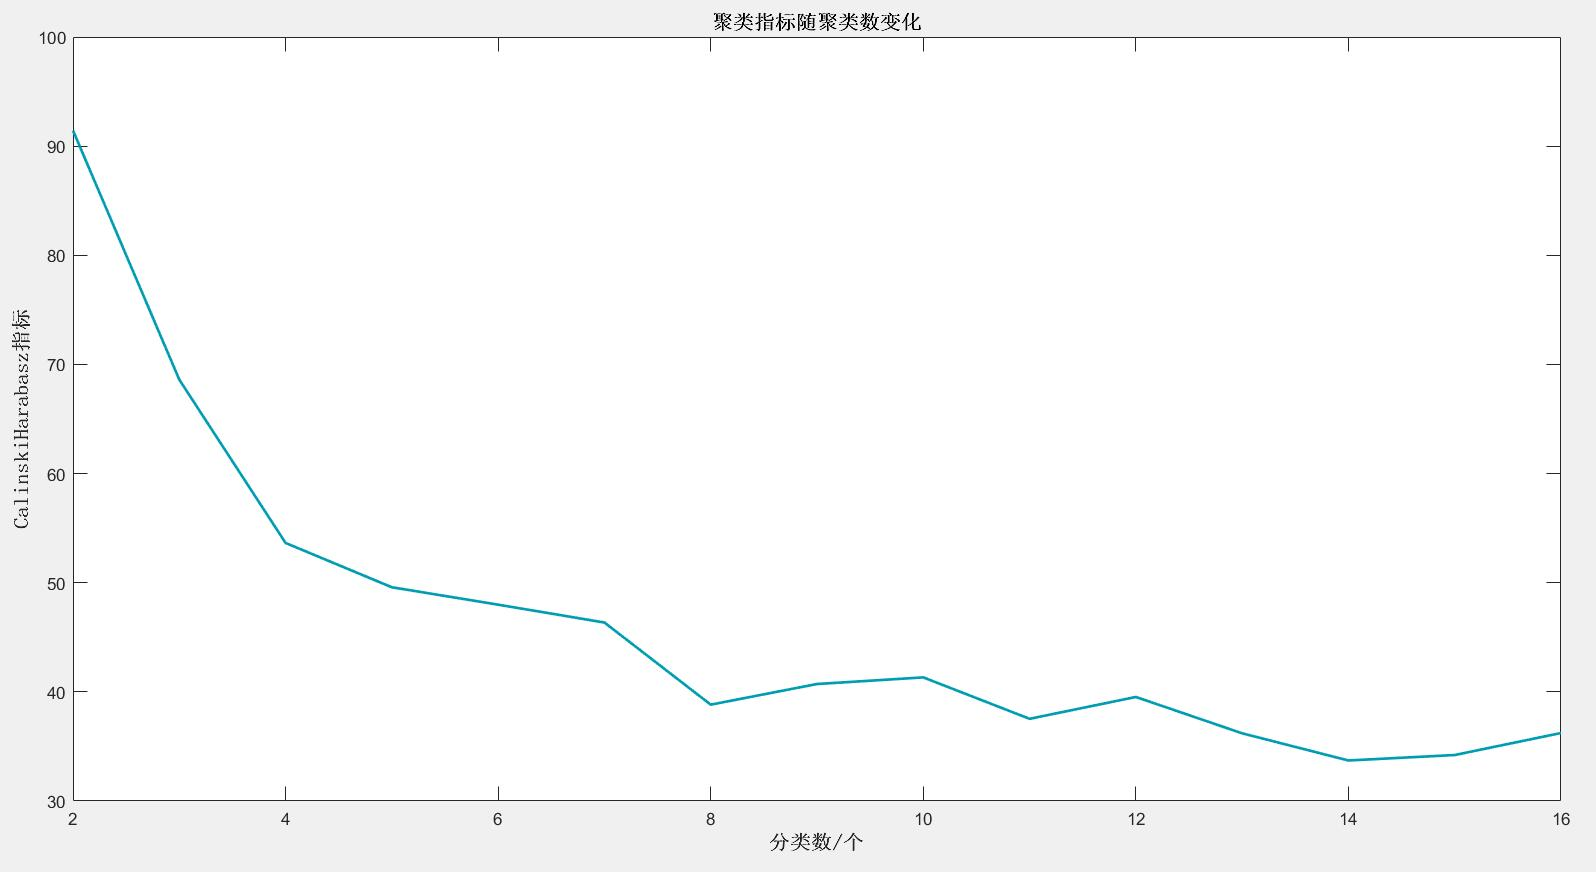
\includegraphics[width=\textwidth]{zhibiao2.jpg}
\caption{不同k值下计算所得的CalinskiHarabasz值} % 标题
\label{zhibiao2}
\end {figure}

最终将用户归为两类:
\begin{itemize}
    \item 类别A:人数131人
    \item 指标: 28个
    
    "1,1,1"	"1,1,2"	"1,1,3"	"1,1,4"	

    "2,2,2"	"2,2,3"	"2,2,5"	"2,2,6"	"2,2,8"	"2,2,9" "2,2,11" "2,2,12"	

    "4,1,1"	"4,1,2"	"4,1,3"	"4,1,4"	"4,1,5"	"4,2,1"	"4,2,2"	"4,2,3"	"4,2,4"	"4,2,5"

    "13,1,11"	"13,1,4"	"13,1,6"	"13,1,7"	"13,1,8"	"13,1,9"

    \item 类别B:人数119 人
    \item 共享指标: 20个
    
    "1,1,1"	"1,1,2"	"1,1,3"	"1,1,4"	

    "4,1,1"	"4,1,2"	"4,1,3"	"4,1,4"	"4,1,5"	"4,2,1"	"4,2,2"	"4,2,3"	"4,2,4"	"4,2,5"

    "13,1,11"	"13,1,4"	"13,1,6"	"13,1,7"	"13,1,8"	"13,1,9"

\end{itemize}
\subsection{基于线性拟合的用户流失时间预测模型}
\subsubsection{线性拟合}
但是其整体的趋势却可以用线性拟合来反映出来,尤其是当其预测的时间段并不长时,其预测精度就更高,趋势形式如持续增高、保持稳定,还是持续下降,持续增高和持续下降就涉及斜率大小,其也可通过线性拟合来决定。

只有一个自变量X的一元线性回归模型是
$$Y=a+bx+\varepsilon ,E(x)=0,D(\varepsilon )=\sigma ^2$$
在这个模型中,a,b为常系数,称为线性回归问题。

\subsubsection{趋势型指标处理}
在前面的模型中,我们将重要指标分成了趋势性指标和数值型指标,趋势性指标我们对其进行滑窗处理,并取其各段斜率的均值作为该指标的“斜率代表”,来作为用户流失打分的依据。
\subsubsection{数值型指标处理}
数值型指标的数值必须在一定范围内才对用户流失有所贡献。所以我们先对已知时间段的数值型指标型数据进行线性拟合,并据此来预测指标的变化情况,即得到未来时间的指标数值。
\subsubsection{用户流失时间段的判断}
我们从当前时间点开始每隔半个月(15天)对数值型指标进行一次提取,同时做一次是否流失的判断。考虑到待预测的用户中有各个用户具有的指标不同,使用直接使用熵权法不能很好的打出一个综合分数。因此,我们还是使用前几问建立的评判模型,之前已经将用户按拥有不同的指标分成了两类,对于待预测用户我们只需根据其拥有的指标将其归到两类之中即可。之后再利用提取出的趋势性指标的“斜率代表”和数值型指标每隔半个月提取的数值套用模型二、三的判断模型,直到用户的分数被定义为“流失”,进而可得到用户流失的大体时间范围。
\section{七、模型的评价}

\subsection{模型的优点}
\begin{enumerate}
    \item 采用滑动窗口法捕捉监控参数的趋势,具有合理性,一定程度上滤除了噪声。
    \item 使用熵权法确定权重,较为客观。

\end{enumerate}

\subsection{模型的缺点}
\begin{itemize}
    \item 数据验证方面尚有不足。

\end{itemize}

%----------- 参考文献 ----------
\newpage
\begin{center}
\bibliography{reference} %调出LaTeX生成参考文献列表
\end{center}

%----------- 附录 ----------
\newpage
\section{附件}
\textbf{附件清单:}
\renewcommand\theenumi{\roman{enumi}}
% 规定数字格式为罗马数字
\renewcommand\labelenumi{\textbf{附录\theenumi}}
% 规定是附录某某
\begin{itemize}
    \item  cluster\_1.m  作用:对用户进行k均值聚类

 
    \item  slide\_main.m 作用:调用滑窗函数分析数据
   
    \item  slide\_win.m   作用:双滑窗法分析数据趋势
    \item  xiangguan.m 作用:指标之间的相关性分析
\end{itemize}




\end{document}